\chapter{Introduction}
\label{chap:intro}
% o General: Start with very general description and focus step by step on your topic
% o keep in mind, that the introduction usually contains the most references
% o Introduction to main topic (e.g. Radiotherapy, MRI, ...) including historical review (1-2pages), Purpose of Radiotherapy ; Regardless of your actual topic, put it in context to conventional photon radiotherapy
% o Basic principles of Physics related to your topic
% o (e.g. Photo effect, Compton effect, Bethe-Bloch equation, ...)
% o Technological Background related to your topic
% o Give a general descriptions about the devices used in your thesis
% o (e.g. Linac, Afterloader, Synchrotron, Detectors...)
% o Overview of literature connected to your topic
% o Purpose of the thesis
% o based on the literature research, describe which information is missing, describe briefly what your thesis is about and what is the novelty of your work

\section{Photon interaction}
\label{sec:photon}
The intensity of light decreases as it travels through matter as described by Beer's law:

\begin{align}
I(x) = I(0) exp[-\mu(h\nu,Z)x]
\end{align}

where x is the thickness of the material,
$\mu$ is the linear attenuation coefficient, which is dependent on the energy of the photons ($h\nu$) and the proton number of the material ($Z$).

The reduction of intensity is due to an number of effects. The photons interaction with electrons (photoelectric effect, Rayleigh scattering, Compton effect), with the electric field of the nuclei (pair production) or with the nuclei itself (photonuclear reactions). The probability of those interactions differ for each material ($Z$) and photon energy ($h\nu$). This behaviour is expressed in the attenuation coefficient $\mu$.


FIGURE WITH ATTENUATION COEFFICIENT


\section{Computer Tomography - CT}

CT is a three-dimensional (3-D) imaging modality based on the measurement of X-ray attenuation.
An X-ray tube emits photons aimed at a receptor positioned on the opposite side of a patient. While travelling through the human body they interact with atoms in various ways (see \ref{sec:photon}). These processes effectively reduce the number of photons reaching the receptor.  Measuring the intensity of the transmitted light corresponds to the projection of attenuation shadows on to the receptor.
As described earlier, the reduction of photons depends on their energy and the tissue (e.g. proton number).
Consequently, the attenuation shadows depict inner structures of the patient, such as bone material.
By mounting source and receptor on a rotary ring with a patient at the centre, images from any angle can be taken. Combining the acquired data results in a 3-D model.

Since its clinical introduction in 1971, computer tomography (CT) has become a widely used 3-D imaging modality for a range of applications including radiation oncology. 



\section{Types of External Beam Radiation Therapy}
External Beam Radiation Therapy (EBRT) utilizes ionizing radiation to damage cancer cells in order to stop them from multiplying.
This prevents the growth of tumours and eventually cures the patient. 
In conventional EBRT photons (x-rays) in the range of 4MeV to 20MeV are used to administer the necessary dose at the location of the tumour. Unfortunately, photons interact with all cells
they're passing through until they are fully stopped. They release their energy slowly while travelling through the patient and usually get completely absorbed after leaving the body.
Charged particles (e.g. protons, carbon ions) minimize the damage done to healthy tissue due to their distinctive behaviour in energy loss called ``Bragg Peak''.
They release most of their energy shortly before stopping. \cite{Nakamura2010} This effect can be used to spare tissue lying behind the tumour from radiation. \cite{Paganetti2005} % and before
A comparison between x-rays and protons is shown in figure \ref{fig:bragg}.

\begin{figure}[!h]
	\centering
	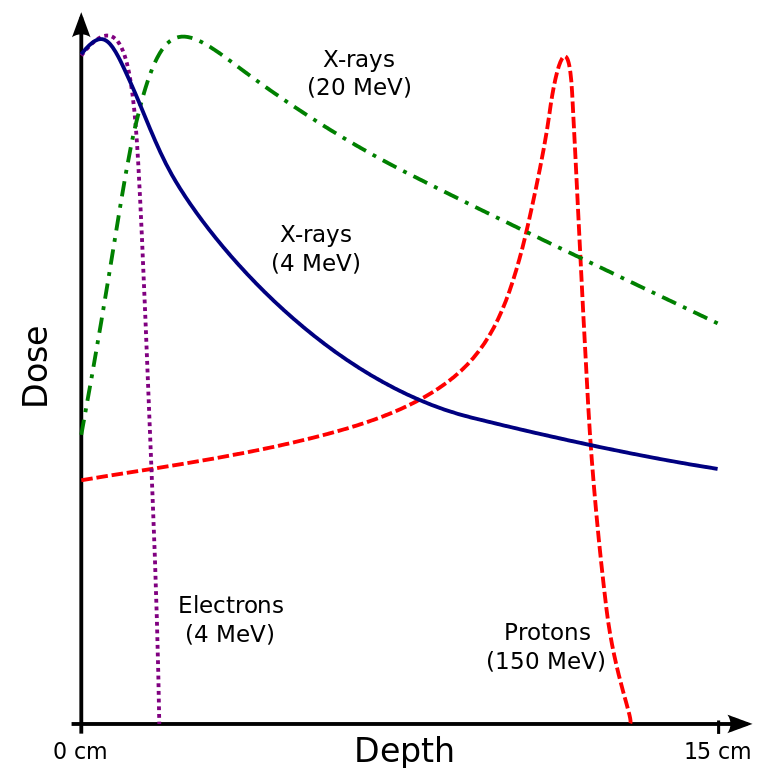
\includegraphics[width=0.6\textwidth]{Dose_Depth_Curves.png}
	\caption{energy release of ionizing radiation \\(By Cepheiden, via Wikimedia Common;\\ GFDL \url{http://www.gnu.org/copyleft/fdl.html})}
	\label{fig:bragg}
\end{figure}

While travelling through matter both types of radiation release energy mostly due to coulomb interactions with the outer shell electrons of atoms.
Knowing the electron density of of the targeted tissue area is therefore essential. In order to reach a specific penetration depth, the particles' initial energy has to be chosen accordingly.

\section{Role of CT}

Until recently radiotherapy treatment planning (RTTP) relied heavily on Computer Tomography (CT). There are two main reasons for this:

Firstly, CT uses low energy x-rays to create a 3D image of the patient. The luminosity value (brightness) assigned to each voxel (like pixel, but three-dimensional) corresponds to
the local radiodensity recorded in Hounsfield units ($HU$). Materials with a higher radiodensity (e.g. bones) absorb more x-ray photons than those with less (e.g. water, brain-mater).
Calculating the electron density using data obtained with CT is an easy task and used widely for RTTP. \cite{Constantinou2012, Schneider1996}
In order not to induce new cancer cells in healthy tissue during EBRT, the radiation beams are carefully targeted using the measured radiodensity. 
This way the absorbed dose accumulates in the cancer regions, while the nearby healthy tissue receives less radiation.

Secondly, CT images generate 3D images with little distortion. Exact geometries are needed for correct RTTP. %more details

\vspace{4cm}
\textit{Image of RTTP}
\vspace{2cm}

\section{Role of MRI}

% mri needs coils
% mri can create differently weighted images (T1, T2, etc..)


Today RTTP often combines CT images with data acquired using Magnetic Resonance Imaging (MRI).
MRI scans also record luminosity values, but they do not correspond to $HU$ (radiodensity measured by CT).
The signal intensity depends on many factors and even varies between MRI scanners.

MRI uses strong stationary magnetic fields to align magnetic spin moments of protons. Then an additional alternating field resonating with the spins is applied shortly to flip them $90^o$.
Depending on the material spins then take longer or shorter to align again with the stationary field. Those differences can be measured in a pick-up coil surrounding the
region of interest. The nature of this effect leads to a great contrast between soft tissue. \cite{Currie2013} Delineating tumours using MRI images is more accurate than using CT.
\cite{Rasch1999, Debois1999a, Roach1996}

Another advantage of MRI over CT is the harmlessness of magnetic fields. CT utilizes the same type of radiation used for destroying cancer cells. Even though the radiation dose of a
CT is low compared to radiation therapy, cancer patients need to be imaged frequently during treatment planning. Especially children treated with EBRT typically
suffer from induced cancer occurring up to 40 years later. So while the benefit from using CT for diagnostics far outweighs the damage, there have been major efforts to
reduce dose while maintaining reasonable image quality. \cite{Murphy2007, Brenner2001, Sodickson2009, Smith2007, McCollough2009, Goldman2013}

There are some difficulties arising from combining CT and MRI for EBRT:
In order to profit from separately acquired data, the resulting images must be aligned either manually or automatically. This is a hard task since non-rigid objects (organs) change their shape and location between measurements. This leads to inaccuracies.
Therefore MRI-only radiation therapy protocols are being developed:
MRI data is used to create a Pseudo-CT, which contains information about electron density. Comparisons to using CT and MRI have shown acceptable deviations for X-ray therapy.
In charged particle therapy the resulting dose gain in healthy tissue and dose loss in cancer regions due to inaccurately assigned electron density values is bigger.
However, current development is promising. \cite{Rank2013, Stanescu2006, Nyholm2015, Greer2015, Chen2004}

\section{Open bore MRI scanners}

% advantages of low tesla, brachytherapy
The radiation oncology department of the Vienna General Hospital (AKH) is equipped with an 0.35T open-bore, c-arm MRI scanner. The open design improves the well-being of patients
experiencing anxiety in closed scanners. Consequently, the number of incomplete MR examinations due to a claustrophobic events is low. \cite{Enders2011a, Bangard2007}
Besides, patients who wouldn't fit in closed designed scanners can be imaged.
Also, brachytherapy patients can be placed in the scanner with applicators attached.

This type of scanner is weaker than a conventional closed bore scanner (1-3 Tesla). High field strengths would result in greater resolution, better Signal to Noise (SNR) ratio, and faster imaging time.
However, ``There are definite cost advantages (capital, operating, siting) to the use of lower field MRI.'' \cite{Rutt1996}
% capital, operating, siting????
Permanent magnets are sufficient to create the 0.35T field. Therefore there is no need for constant cooling using liquid helium compared to superconducting magnets.
Consequently, maintenance and service costs are considerably lower.

Generally, diagnostics benefit from greater image quality. However, at some point diagnostic accuracy stops increasing with field strength.
Nevertheless, high field scanners are key to developing new methods such as functional MRI (fMRI) of the brain \cite{Duyn2012} and observing
``metabolic reactions occurring in a human body in addition to producing very precise images of body structures'' \cite{Wada2010}.
At the same time astonishing improvements can be achieved at low fields.
A ``combination of field independent polarization [...] with frequency optimized MRI detection coils [...] results in low-field MRI sensitivity approaching and even rivaling that of high-field MRI.'' \cite{Coffey2013}

One drawback of MRI, and especially open bore scanners, is the occuring distortion due to inhomogeneities in the magnetic field.
For most applications small position shifts and deformations are of minor importance. In RTTP however, those effects can have a big impact.
Therefore MRI scanners usually come equipped with an internal distortion correction algorithm.
Those methods are developed by the company designing the scanners. Knowing the technical details enables them to drastically reduce the distortion.

Field of view (FOV) of the MRI scanner is smaller than the CT scanner's.

\section{Aim of this work}
The used open bore MRI scanner is not intended to be used for RTTP. The on board correction algorithm might not be good enough for effetive EBRT.
The goal of this work is to commence the development of a quality assurance tool to asses the spatial distortion (after applying the internal correction).
This is achieved by comparing MRI images to CT images used as a gold standard.
An alerady existing custom designed phantom is provided by the AKH Vienna for this purpose.
However, the liquid to fill the rods with has not been chosen yet.
Therefore, this paper focuses mainly on the acquired data and which liquids to use the phantom with, not its entire design.
However, possible fillings have to be produced and tested.
Similar approaches are being used for distortion correction by other facilities. \cite{Price2015, Petersch2004, Torfeh2015, Wang2004, Wang2004b, Mizowaki2000}


%to me \footnote{Auszug aus \citetitle{BohemRhap}~\cite{BohemRhap} von \citeauthor{Queen}~\cite{Queen} }\\
%\section{Farrokh Bulsara aka. Freddie Mercury}
%Farrokh Bulsara war ein Ausnahmetalent schuf zusammen mit der Band Queen einige der größten Hits aller Zeiten. Noch heute ist er ein wichtiges Thema in unterschiedlichsten Medien, wie in Abb. \ref{fig:freddiehg} zu sehen ist. %
%Weitere Zitate sind in Anhang \ref{appendix:zitate} zu finden.


\newpage